% Compile with XeLaTeX or Tectonic. No shell escape or external images required.
\documentclass[10pt,a4paper]{article}
\usepackage[margin=18mm,headheight=15pt,headsep=8mm,footskip=10mm]{geometry}
\usepackage{fontspec}
\setmainfont{texgyreheros-regular.otf}[BoldFont=texgyreheros-bold.otf,ItalicFont=texgyreheros-italic.otf]
\usepackage[table]{xcolor}
\usepackage{tabularx,booktabs,array,enumitem,titlesec,fancyhdr,tikz}
\usetikzlibrary{arrows.meta,positioning}
\usepackage[colorlinks=true,urlcolor=teal,linkcolor=teal]{hyperref}
\definecolor{navy}{HTML}{17343D}
\definecolor{teal}{HTML}{087F82}
\definecolor{mint}{HTML}{EAF5F2}
\definecolor{muted}{HTML}{53666D}
\definecolor{coral}{HTML}{C65D47}
\hypersetup{pdftitle={ZentroMart AI Support Agent},pdfauthor={Mrinal Subudhi}}
\pagestyle{fancy}\fancyhf{}
\fancyhead[L]{\small\color{teal}\textbf{ZENTROMART} / VOICEOPS 2026}
\fancyhead[R]{\small\color{muted}Mrinal Subudhi}
\fancyfoot[L]{\footnotesize\color{muted}Capstone report | 1 November 2026}
\fancyfoot[R]{\footnotesize\color{teal}\thepage\ / 4}
\renewcommand{\headrulewidth}{0.4pt}
\titleformat{\section}{\large\bfseries\color{navy}}{}{0pt}{}
\titleformat{\subsection}{\normalsize\bfseries\color{teal}}{}{0pt}{}
\titlespacing*{\section}{0pt}{10pt}{5pt}
\titlespacing*{\subsection}{0pt}{8pt}{4pt}
\setlength{\parindent}{0pt}\setlength{\parskip}{5pt}
\setlength{\emergencystretch}{2em}
\setlist[itemize]{leftmargin=14pt,itemsep=3pt,topsep=3pt}
\renewcommand{\arraystretch}{1.18}
\newcommand{\tagline}[1]{{\small\bfseries\color{teal}#1}\par}
\newcommand{\note}[1]{\par\noindent\colorbox{mint}{\parbox{\dimexpr\linewidth-2\fboxsep}{\small #1}}\par}
\newcommand{\repo}{\href{https://github.com/brindoxx/ZentroMart-AI-Support-Agent}{github.com/brindoxx/ZentroMart-AI-Support-Agent}}
\begin{document}
\tagline{DOCUMENT-GROUNDED SUPPORT, WITH A VOICE}
{\fontsize{27}{31}\selectfont\bfseries\color{navy}ZentroMart AI\par Support Agent}\par
{\large\color{muted}Mrinal Subudhi | Individual submission}\par
\textbf{Repository:} \repo

\section{Problem and approach}
ZentroMart is a fictional Indian retailer. A useful support assistant must explain
its policies, handle follow-ups and avoid inventing order outcomes. I built a
text and voice application that combines Gemini conversation planning, hybrid
document retrieval, deterministic order workflows and Gnani speech services.
The implementation uses Streamlit and custom Python rather than an agent framework.

\note{Design boundary: the LLM proposes language and next steps; application code
controls verification, calculations and tools. A fluent answer is not evidence
that a refund, cancellation or handover actually happened.}

\section{Data and architecture}
The supplied synthetic dataset contains 21 knowledge documents, 9 CSVs, 1,000
orders, 1,783 order items and 244 historical logs. Evaluation material includes
52 questions and 23 conversations with 96 customer turns. Retrieval uses 154
public sections/catalog records; private customer/order tables are not embedded.
The calculation reference date remains 20 October 2026, not the computer's date.

\begin{center}
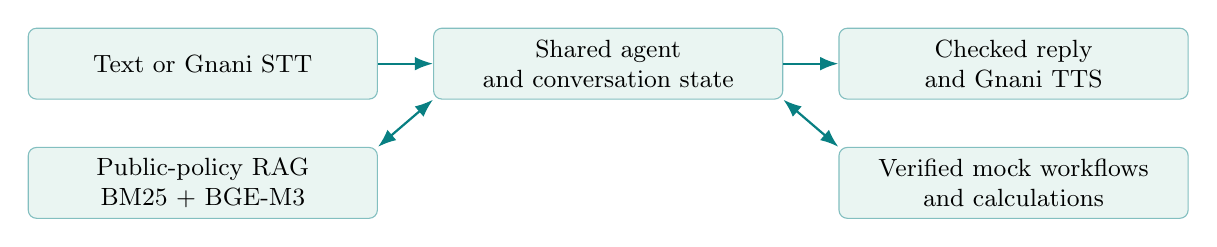
\begin{tikzpicture}[node distance=6mm and 7mm,>=Latex,
 box/.style={draw=teal!50,fill=mint,rounded corners=3pt,align=center,font=\small,minimum height=9mm,text width=42mm},
 arrow/.style={->,thick,draw=teal}]
\node[box] (in) {Text or Gnani STT};
\node[box,right=of in] (agent) {Shared agent\\and conversation state};
\node[box,right=of agent] (out) {Checked reply\\and Gnani TTS};
\node[box,below=of in] (rag) {Public-policy RAG\\BM25 + BGE-M3};
\node[box,below=of out] (tools) {Verified mock workflows\\and calculations};
\draw[arrow] (in)--(agent);\draw[arrow] (agent)--(out);
\draw[<->,thick,draw=teal] (agent.south west)--(rag.north east);
\draw[<->,thick,draw=teal] (agent.south east)--(tools.north west);
\end{tikzpicture}
\end{center}

\section{Step 1 / Establish a real LLM baseline}
The prompt-only adapter sends Gemini a support-role prompt and the current
question without documents, tools, history or gold labels. This is distinct from
the offline wiring baseline that always clarifies. Both live comparison arms
used the same requested model, \texttt{gemini-3.5-flash-lite}, and 52 questions.

\section{Step 2 / Ground answers in documents}
Ingestion preserves section IDs, source paths, status and effective dates.
BM25 and normalized dense cosine search feed reciprocal-rank fusion. Policy
precedence and scenario applicability determine the evidence bundle; Gemini
answers from that bundle. Citation-ID guards reject invalid drafts and return a
safe fallback. They do not establish semantic entailment or perfect grounding.

\newpage
\tagline{IMPLEMENTATION / CONVERSATION AND VOICE}
\section{Step 3 / Keep one conversation and control actions}
The shared \texttt{create\_agent} factory is used by the UI, CLI, evaluation and
batch audio runner. Each conversation owns its memory, verification and tool
state. ASGI startup preloads public documents, the calendar and the selected
query encoder with a fixed public warm-up search. The UI reuses bounded caches;
no provider request, credential-bearing client or private state is warmed.
CPU encoder access is serialized.
Gemini proposes structured actions: answer, clarify, search or enter a supported
workflow. The application validates the proposal before dispatching it.

English, Hindi and Hinglish replies follow the current turn. Conversation context
supports follow-ups such as identifying an item and then supplying its delivery
timing. Verification and active private steps can remain local; not every message
needs an LLM call. Bounded history and per-session budgets limit cost and exposure.

\subsection{Private workflow boundary}
Order details require an eight-digit order ID and a separate typed phone suffix
or pincode in a masked field. This is synthetic mock verification, not production
authentication. Verified order records and proofs are excluded from the Gemini
dialogue prompt. Backend code calculates policy estimates and invokes allowlisted
mock tools; it cannot issue real refunds or cancel orders.

\note{The sidebar's demo-ticket permission only enables local mock ticket writes.
A handover must still be requested and the executor must confirm creation. It
does not approve a refund, notify a real team or create a ticket when toggled.}

\section{Step 4 / Use Gnani for listening and speaking}
The application uses Gnani WebSocket STT and Gnani TTS model
\texttt{timbre-v2.5}, with no alternate speech provider or browser speech fallback.
The mic button prepares an editable transcript; voice mode submits completed
speech turns, plays the agent's reply and resumes listening afterwards. This is
sequential voice interaction, not full-duplex or barge-in support.

The batch runner accepts a WAV folder. A manifest can group ordered files into
one conversation; otherwise each file gets an independent session. It converts
16-bit PCM mono/stereo WAVs to 16-kHz mono in memory. Current capture/input limits
are 15 seconds per file; long TTS replies are chunked without silent truncation.
Every result records its stage, safe failure code and whether speech was actually
generated. Dependent turns are skipped after a failed conversation turn.

\subsection{Safety, consent and recoverability}
\begin{itemize}
\item Cloud processing requires explicit consent in the UI; batch processing
requires \texttt{--live}. Only synthetic content and the owner's consented test voice are used.
\item Voice pauses for typed verification. The batch runner blocks pending proof
collection instead of processing a spoken proof as verification.
\item Failed requests count toward budgets. The measured batch used no automatic
retries. Authentication/quota failures stop remaining batch requests.
\item First returned replies explicitly disclose AI identity in the shared
controller and browser boundary; text, voice and batch paths have offline tests.
ISO dates and labelled order IDs are reformatted only for speech, without changing written facts.
\end{itemize}

\subsection{Enhancements beyond the minimum}
The project adds automatic reply-language switching, guided invented demo orders,
per-turn source inspection, deterministic estimates and a reproducible local
encoder/reranker comparison. These extras do not replace the required grounded
conversation, audio runner and measured baseline comparison.

\newpage
\tagline{MEASURED EVIDENCE / NOT AN OVERALL ACCURACY CLAIM}
\section{Step 1 versus Step 2}
Measured on 31 October 2026. Both arms completed 52/52 original-text practice
questions: 104 generation attempts and zero provider/adapter errors. The RAG arm
used \textbf{E5-small and grounded prompt v3}, not the later BGE configuration.
The comparison is stateless and does not score the full conversation controller.

{\small
\begin{tabularx}{\linewidth}{@{}Xrr@{}}
\toprule
\rowcolor{mint}\textbf{Metric} & \textbf{Prompt-only} & \textbf{E5 hybrid RAG}\\
\midrule
Decision agreement (52 cases) & 32.7\% (17/52) & 48.1\% (25/52)\\
Required-fact lexical coverage (49 cases) & 12.2\% & 38.8\%\\
Declared language agreement & 86.5\% (45/52) & 94.2\% (49/52)\\
Retrieval Hit@5 (47 gold-evidence cases) & No retrieval & 83.0\% (39/47)\\
Retrieval Recall@5 & No retrieval & 55.7\%\\
Citation precision (35 cited RAG responses) & N/A & 76.7\%\\
Citation recall (47 cases) & 0\% & 39.4\%\\
\bottomrule
\end{tabularx}}

RAG returned 44 accepted generated answers and \textbf{8 citation-mismatch safe
fallbacks}. Decision agreement checks the chosen action, not every factual claim.
Lexical coverage can miss valid paraphrases or accept misleading wording.
Citation scores compare source IDs, not entailment. No forbidden-claim lexical
hits occurred in eight labelled cases; that is not a general safety guarantee.

\section{Which retriever should the final app use?}
Local CPU tests kept chunking, BM25 and rank fusion unchanged. Each input variant
has 47 scored questions. ASR-like variants are supplied text, not new STT outputs.
No Gemini/Gnani calls were used for this experiment.

{\small
\begin{tabularx}{\linewidth}{@{}Xrrr@{}}
\toprule
\rowcolor{mint}\textbf{Hybrid configuration} & \textbf{Text Hit@5} & \textbf{ASR Hit@5} & \textbf{Warm search}\\
\midrule
E5-small & 83.0\% & 78.7\% & 32 ms\\
\rowcolor{mint}BGE-M3 (selected) & 87.2\% & 83.0\% & 246--271 ms\\
E5 + MiniLM cross-encoder & 76.6\% & 70.2\% & 1.68--1.70 s\\
BGE + MiniLM cross-encoder & 76.6\% & Not run & 1.80 s\\
\bottomrule
\end{tabularx}}

BGE-M3 improved top-five hits by two questions per input variant; text Recall@5
rose from 55.7\% to 57.8\%. The tested multilingual MiniLM cross-encoder reranked
20 candidates but reduced coverage, so it is implemented and \textbf{disabled by
default}. BGE uses 1,024-dimensional CLS-pooled dense vectors; E5 uses
384-dimensional mean-pooled vectors. Both used a 512-token maximum.
Warm timings exclude downloads/loading; overlapping CPU work makes them approximate.

\section{Voice and regression evidence}
Six real recordings across three cases completed STT, agent processing and TTS:
\textbf{6 Gemini generations, 12 Gnani requests, no retries and no failed/skipped
turns}. The four-turn case retained item context and changed from English to
Hindi before requesting an order ID. The owner listened to the generated replies
and reported satisfactory speech. This is a small subjective check, not WER or a
general voice-reliability score. The offline suite passed \textbf{339 tests},
including 11 batch-audio, four release, ten conversation/presentation and four startup checks.

An approved four-turn text rehearsal of the revised demo also completed:
AI-disclosed greeting, cited damage-policy answer, context-aware pickup answer
and executor-confirmed mock handover. It used five Gemini generations and zero
speech requests; both policy drafts passed on the first attempt. This is a small
live text check, not an accuracy benchmark or a new voice recording.

\newpage
\tagline{LIMITATIONS / REPRODUCIBILITY / NEXT STEPS}
\section{What went wrong and what I learned}
\begin{itemize}
\item \textbf{Grounding is still imperfect.} Eight citation fallbacks and missing
facts remain. I would inspect wrong decisions and passage support, improve
language-aware evaluation and test full conversations before claiming accuracy.
\item \textbf{More components did not automatically help.} The cross-encoder was
slower and worse on these labels. I kept the measured simpler configuration.
NumPy exact cosine matched SciPy; a database migration was not an accuracy fix.
\item \textbf{An obsolete capability instruction leaked into a reply.} The saved
damage answer says lookup was not connected. Review identified the old public
prompt instruction; v4 corrects it. Samples remain unchanged, and neither the
historical answer benchmark nor the six-file live run was repeated after this fix.
\item \textbf{Follow-ups exposed a retrieval gap.} The planner saw history, but
search used only the latest sentence. The shared controller now includes bounded
public customer context in retrieval. One citation-correction generation is
allowed after a reference failure; the same guards still apply. Invalid second
drafts are withheld with a safe diagnostic and recovery prompt. This exact
damage/pickup/handover exchange passes controlled offline tests, not a new live benchmark.
\end{itemize}

\section{Reproduce and inspect the solution}
Obtain the course dataset separately and point \texttt{DATASET\_DIR} at its
extracted \texttt{kb/}, \texttt{data/}, \texttt{practice/} and \texttt{tools/}
folders. Create a Python 3.11+ environment, install \texttt{requirements.txt}, copy
the key-free template to \texttt{.env}, and add local Gemini/Gnani keys.
The first retrieval run downloads its pinned public encoder; keys and model
weights are not included in the submission.

\note{\textbf{Batch command, from the repository root:}\par
\texttt{python run.py audio\_samples --manifest audio\_cases.json --live}\par
Add \texttt{--offline} only after the encoder is cached. Omitting \texttt{--live}
runs local WAV/manifest preflight only.}

Each run creates a unique output folder with \texttt{summary.json}, model usage
and numbered turn directories containing reply text, reply WAV, public source
chunks and safe status. Missing/failed speech is reported explicitly. The live
examples are in \texttt{sample\_outputs/audio\_demo}; input recordings and the
ordered case manifest are included with the owner's permission.

Default batch limits are 24 model generations, 30 speech requests, five-second
model pacing and a conservative 250,000-input-TPM guard. The browser has its own
budgets. These controls do not discover remaining project-wide account quota.
The original 52-question experiment used user-reported 15 RPM / 250k TPM / 500 RPD
limits and no retries; another run consumes additional quota.

The release may spend one extra generation on citation correction; successful
first drafts cost no extra call, and quota/provider errors are not retried by
that mechanism. Wider voice/noise testing, clearer provider-error recovery and a
truly clean-machine install remain limitations. Missing date years are not guessed.

\subsection{Where to verify the evidence}
\textbf{Code and setup:} \repo\par
\textbf{Answer metrics:} \texttt{evals/results.md}; includes denominators,
historical prompt hash and reproduction caveats.\par
\textbf{Retriever selection:} \texttt{evals/retrieval-experiments.md}; pinned
model revisions, recall/MRR and local report IDs.\par
\textbf{Recorded examples:} \texttt{sample\_outputs/README.md}; real outcomes,
known sample wording issue and owner listening review.\par
\textbf{Checks:} \texttt{python -m unittest discover -s tests -q} and
\texttt{node tests/composer\_frontend.mjs}.

\note{This is an educational synthetic-data application. No fine-tuning was
performed; practice labels were not used as training data or agent context.
Performance is development-set evidence, not held-out accuracy or production
readiness. The final demo and clean-install check are release gates.}
\end{document}
